% Risk Lab: overfitting study of the UFOS validation gates - draft.
% Figures and tables are generated by report/build_report.py --doc overfitting (synthetic data only).
% Every \usertext{...} is an open prose slot for the author; a build with open slots is a draft.
% Required LaTeX packages (checked by build_report.py): geometry, graphicx, xcolor, booktabs, array,
% amsmath, amssymb, caption, float, hyperref. Fonts: Computer Modern (no lmodern needed).
\documentclass[11pt,a4paper]{article}
\usepackage[a4paper,margin=2.3cm]{geometry}
\usepackage{graphicx}
\usepackage[dvipsnames]{xcolor}
\usepackage{booktabs}
\usepackage{array}
\usepackage{amsmath,amssymb}
\usepackage{caption}
\usepackage{float}
\usepackage[hidelinks]{hyperref}
\captionsetup{font=small,labelfont=bf}
\graphicspath{{./}}

% Reproducible PDF: no creation date, empty trailer ID (pdfTeX primitives).
\ifdefined\pdfinfoomitdate \pdfinfoomitdate=1 \fi
\ifdefined\pdftrailerid \pdftrailerid{} \fi

% ---- open text slots ---------------------------------------------------------------
\newcounter{usertextslots}
\newcommand{\usertext}[1]{%
  \stepcounter{usertextslots}%
  \par\medskip\noindent
  \fcolorbox{BurntOrange}{Goldenrod!18}{\parbox{\dimexpr\linewidth-2\fboxsep-2\fboxrule\relax}{%
    \small\textbf{\textcolor{BurntOrange}{TEXT SLOT \theusertextslots:}} \textit{#1}}}%
  \par\medskip}
\makeatletter
\AtEndDocument{\immediate\write\@auxout{\string\gdef\string\totalusertextslots{\theusertextslots}}}
\makeatother
\providecommand{\totalusertextslots}{?}

\title{How often does an overfitted rule pass the UFOS validation gates?\\[0.3em]
  \large A Monte-Carlo study of false positives, power and the holdout on synthetic data}
\author{}
\date{}

\begin{document}
\maketitle
\vspace{-2em}
\usertext{Author, function and date of the study.}
\begin{center}
\fcolorbox{BrickRed}{BrickRed!8}{\parbox{0.9\linewidth}{\centering\small
\textbf{DRAFT} -- this version has \totalusertextslots{} open text slots (orange boxes).
All figures and tables are generated from synthetic data by \texttt{report/build\_report.py --doc overfitting}.}}
\end{center}
\tableofcontents

% =====================================================================================
\section{Executive summary}
The UFOS strategy platform lets a strategy trade only after it has passed the validation gates G1--G8 on
its training data and the holdout gate H on the last 24 months (SPEC \S 9). The gates are meant to stop
rules that look good only because many variants were tried. This study measures, on synthetic data with a
known truth, how often the best of $K$ searched configurations of a simple trend rule passes the gates when
the rule has no edge (the false-positive rate), how often it passes when the rule has a real edge (the
power), and what the holdout adds. The gate statistics are re-implemented independently in Risk Lab and
checked against the platform's code by a parity test.

The findings are listed in Table~\ref{tab:O6_findings}; their severities are proposals.
\usertext{The overall conclusion in two or three sentences: are the gates conservative enough, and is the
price in power acceptable for the intended use? Refer to the findings by ID.}

% =====================================================================================
\section{Question and scope}
Question: when a user searches over $K$ parameter configurations of a rule and validates the best one,
\begin{itemize}
\item how often does a rule \emph{without} an edge pass each gate alone, all in-scope gates together, and
  those together with the holdout (false-positive rate, FPR)?
\item how often does a rule \emph{with} a real edge pass (power), as a function of its true Sharpe ratio,
  the training length and the preset?
\item does the holdout gate improve the decision beyond the training gates?
\item do the calibration claims of SPEC \S 9.6 hold (``at least 95\,\% of noise seeds fail at least one
  gate''; ``best-of-64 noise fails G4 or G5'')?
\end{itemize}

\paragraph{Gates in scope.} Table~\ref{tab:O1_gates_scope} lists the gates, the rule each implements in
UFOS, what this study covers and the thresholds of the three presets. In scope are G1 in its
time-series form (fold Sharpe $>0$ in at least $n$ of five walk-forward folds), G2 (alpha against the
benchmark with a Newey--West $t$), G4 (the deflated Sharpe ratio), G5 (the probability of backtest
overfitting by CSCV over the parameter grid), the grid-neighbour part of G6, G7 (the number of closed
trades) and H.

\paragraph{Out of scope.} G1's cross-sectional rank-IC form (the study's rule trades a single asset);
G3 (signal decay, ``not applicable'' to single-asset rules in UFOS, where it counts as a pass); the
cost-multiplier and stress-episode parts of G6; and G8 (capacity). The results below therefore describe
the in-scope gates only. For a single-asset rule in UFOS, G3 passes by rule, so the platform's decision can
differ from the in-scope result only through the G6 cost and episode checks and G8 (not applicable, and
passed, for crypto-only universes).

\begin{table}[H]
\centering
\scriptsize
\caption{The UFOS validation gates (SPEC \S 9.4), what this study covers, and the preset thresholds. Out of scope: G1's cross-sectional rank-IC form, G3, the cost and stress parts of G6, and G8.}
\label{tab:O1_gates_scope}
\setlength{\tabcolsep}{3pt}
\begin{tabular}{>{\raggedright\arraybackslash}p{0.75cm}>{\raggedright\arraybackslash}p{1.7cm}>{\raggedright\arraybackslash}p{5.1cm}>{\raggedright\arraybackslash}p{2.3cm}lll}
\toprule
Gate & Name & UFOS rule & This study & Lenient & Standard & Strict \\
\midrule
G1 & Consistency & time-series: fold Sharpe $> 0$ in $\ge n$ of 5 walk-forward folds; cross-sectional: rank-IC NW $t$ and fold mean IC & time-series form & 3 of 5 & 4 of 5 & 5 of 5 \\
G2 & Alpha & OLS alpha vs the benchmark $> 0$ and its Newey-West $t \ge$ threshold & vs buy and hold of the asset & $t \ge$ 1.5 & $t \ge$ 2 & $t \ge$ 3 \\
G3 & Signal decay & IC half-life $\ge$ average holding period (single-asset: not applicable) & out of scope & -- & -- & -- \\
G4 & Deflated Sharpe & DSR with $N$ = trials + 1, trial-Sharpe variance floored at 1/years & $N = K + 1$ & $\ge$ 0.90 & $\ge$ 0.95 & $\ge$ 0.99 \\
G5 & Overfitting (PBO) & CSCV, $S = 10$ blocks, over the parameter grid ($\le 64$); $< 4$ configurations fail & 64-configuration UFOS grid & $\le$ 0.50 & $\le$ 0.30 & $\le$ 0.20 \\
G6 & Robustness & (a) grid neighbours ($\pm$20\,\%) keep $\ge r\times$ the base Sharpe; (b) costs $\times m$ stay profitable; (c) stress-episode drawdowns & (a) only & $r$ = 0.40 & $r$ = 0.50 & $r$ = 0.60 \\
G7 & Sample size & closed trades $\ge n$ & position changes & $\ge$ 50 & $\ge$ 100 & $\ge$ 200 \\
G8 & Capacity & capacity estimate $\ge$ 10 $\times$ the tested capital & out of scope & -- & -- & -- \\
H & Holdout & holdout Sharpe $> 0$ and $\ge$ 50\,\% of the training Sharpe (fixed) & last 24 months, once & fixed & fixed & fixed \\
\bottomrule
\end{tabular}
\end{table}

\usertext{Why these gates and presets were chosen for the first study, and which of the out-of-scope parts
should be studied next.}

% =====================================================================================
\section{Design}
\subsection{Rule family and search}
A moving-average crossover on the log price $x_t$: the position decided at the close of day $t$ and held on
day $t+1$ is $p_t = \operatorname{sign}(\mathrm{MA}_{f}(x)_t - \mathrm{MA}_{s}(x)_t) \in \{-1, +1\}$ (long or
short). The parameters are \texttt{fast} $f \in \{4,\dots,19\}$ (step 1) and \texttt{slow}
$s \in \{24, 27, \dots, 69\}$ (step 3), written as UFOS DSL parameters with \texttt{min}, \texttt{max} and
\texttt{step}: $16 \times 16 = 256$ configurations, the search space. Under noise the rules change position
about 7 to 18 times a year.

The user tries $K \in \{1, 8, 64, 256\}$ configurations, the first $K$ of a random permutation of the 256
(the same permutation for every $K$, so the searches are nested on the same data; $K = 1$ is one random
configuration), and validates the one with the best training net Sharpe ratio. The UFOS grid of the
validated specification has the same \texttt{min}/\texttt{max}/\texttt{step} with the selected values: 256
configurations, which the platform subsamples evenly to 64 with the selected (base) configuration forced
in. G5 and G6 run on these 64.

\subsection{Data}
Daily returns $r_t = \mu\, q_{t-1} + \varepsilon_t$ with an annual volatility of 20\,\%, where $q_{t-1}$ is
the position of the \emph{true} configuration ($f = 8$, $s = 42$), computed sequentially from the
simulated prices up to $t-1$, and $\mu = \mathrm{SR}\cdot\sigma_d/\sqrt{252}$, so that the true configuration
earns a gross Sharpe ratio of $\mathrm{SR} \in \{0, 0.25, 0.5, 0.75, 1.0\}$ a year ($\mathrm{SR} = 0$:
pure noise, no configuration has an edge). The innovations $\varepsilon_t$ are standardised Student-$t$
($\nu = 5$), either iid or with GARCH(1,1) volatility ($\alpha = 0.08$, $\beta = 0.90$, unconditional
variance $\sigma_d^2$). The training sample has 5, 10 or 20 years of 252 days; the following 504 days (24
months) are the holdout, evaluated once for the selected configuration. Within a (data, length) cell all
signal levels share the innovations and the search order (common random numbers), so the power curves are
smooth in the signal.

Costs of 2 basis points per unit of turnover are deducted (a flip from long to short is two units); every
position change closes a trade (G7). The benchmark of G2 is buy and hold of the asset.

\subsection{Gate inputs}
The selected configuration's training net returns feed the gates as the platform's validation job does
(SPEC \S 9.3): G1 the Sharpe ratios of five consecutive folds of equal length; G2 the OLS alpha against the
benchmark with a Newey--West standard error (Bartlett kernel, lag $L = \lfloor 4 (T/100)^{2/9} \rfloor$,
Newey and West 1994; small-sample factor $T/(T-k)$); G4 the deflated Sharpe ratio (Bailey and L\'opez de
Prado 2014) with $N = K + 1$ trials and the variance of the trials' annualised Sharpe ratios (the $K$
training Sharpe ratios plus the validated run's), floored at $1/\text{years}$; G5 the PBO by CSCV with
$S = 10$ blocks and $\binom{10}{5} = 252$ splits (Bailey, Borwein, L\'opez de Prado and Zhu 2017), a split
counting as overfit when the logit of the in-sample winner's relative out-of-sample rank is $\le 0$; G6
the grid neighbours within $\pm 20\,\%$ of every parameter, each of which must keep at least the preset
share of the base Sharpe ratio; G7 the number of closed trades; H the holdout net Sharpe ratio ($> 0$ and
$\ge 50\,\%$ of the training Sharpe ratio). A gate whose statistic cannot be computed fails, as in UFOS.

We report the in-scope gates together (G1, G2, G4, G5, G6, G7) and the \emph{statistical} gates (the same
without G7): G7 depends on the rule's trading frequency and the sample length rather than on the search,
and it alone would decide the five-year results.

\subsection{Re-implementation and parity}
\texttt{risklab.validation} re-implements the statistics and gate rules from the SPEC and the papers and
does not import the platform. The HedgeFund-side test \texttt{test\_risklab\_gate\_parity.py} (in
\texttt{HedgeFund/backend/tests}) compares both implementations on fixed synthetic inputs: Sharpe ratio, moments, PSR, the expected maximum Sharpe
ratio, DSR, PBO, the Newey--West regressions, the fold bounds, the grid (axes, the 64-configuration
subsample with the forced base, the neighbours) and 900 gate decisions over the three presets. All agree
(numbers to $10^{-9}$, PBO and decisions exactly).

\subsection{Monte-Carlo design}
$M$ paths per (data, training length, signal) cell; every rate carries the binomial standard error
$\sqrt{p(1-p)/M}$ (conditional rates: on the $n$ conditioning paths). The full run uses $M = 2000$
(seed 20261109); the results file records the code fingerprint, and the report build refuses stale
results.
\usertext{Comment on the design choices that matter most for the conclusions (rule family, cost level,
the true configuration inside the search space, $N = K + 1$).}

% =====================================================================================
\section{Results}
\subsection{False positives under noise}
\begin{figure}[H]
\centering
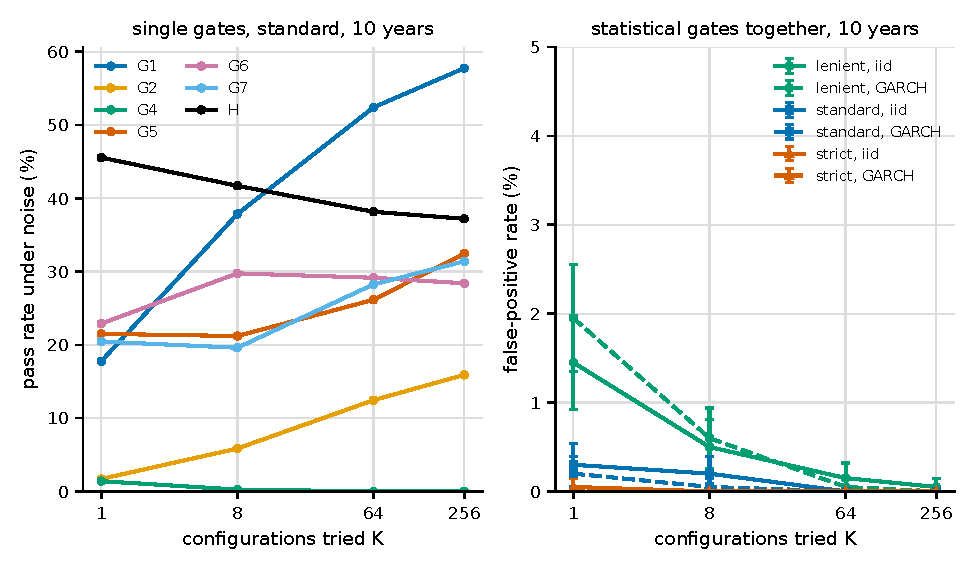
\includegraphics[width=\linewidth]{figures/fig8_fpr_vs_k.pdf}
\caption{Pass rates of the best of K configurations under noise (true Sharpe 0), 10 training years, M = 2000 paths per cell. Left: each gate alone (standard preset, iid $t_5$ data; Monte-Carlo se at most 1.1 percentage points). Right: the statistical gates together (G1, G2, G4, G5, G6 neighbours) per preset; solid iid, dashed GARCH, error bars $\pm 1.96$ se.}
\label{fig:fig8_fpr_vs_k}
\end{figure}

\begin{table}[H]
\centering
\scriptsize
\caption{False-positive rate (\%) under noise (true Sharpe 0) of the best of $K$ configurations: statistical gates (G1, G2, G4, G5, G6 neighbours) per preset, with H, and all in-scope gates (with G7) for the standard preset. M = 2000 paths per cell, $\pm$ Monte-Carlo se; a rate of 0 or 100 shows the 95\,\% bound of the rule of three in brackets (3 / n).}
\label{tab:O2_fpr}
\setlength{\tabcolsep}{3pt}
\begin{tabular}{lrrrrrrrr}
\toprule
Data & Years & $K$ & Stat.\ L & Stat.\ S & Stat.\ St & Stat.\ S + H & All S & All S + H \\
\midrule
iid $t_5$ & 5 & 1 & 1.8 $\pm$ 0.3 & 0.4 $\pm$ 0.1 & 0.1 $\pm$ 0.0 & 0.2 $\pm$ 0.1 & 0 ($\le$ 0.15) & 0 ($\le$ 0.15) \\
iid $t_5$ & 5 & 8 & 0.6 $\pm$ 0.2 & 0 ($\le$ 0.15) & 0 ($\le$ 0.15) & 0 ($\le$ 0.15) & 0 ($\le$ 0.15) & 0 ($\le$ 0.15) \\
iid $t_5$ & 5 & 64 & 0.1 $\pm$ 0.1 & 0 ($\le$ 0.15) & 0 ($\le$ 0.15) & 0 ($\le$ 0.15) & 0 ($\le$ 0.15) & 0 ($\le$ 0.15) \\
iid $t_5$ & 5 & 256 & 0.1 $\pm$ 0.1 & 0 ($\le$ 0.15) & 0 ($\le$ 0.15) & 0 ($\le$ 0.15) & 0 ($\le$ 0.15) & 0 ($\le$ 0.15) \\
\midrule
iid $t_5$ & 10 & 1 & 1.5 $\pm$ 0.3 & 0.3 $\pm$ 0.1 & 0.1 $\pm$ 0.0 & 0 ($\le$ 0.15) & 0 ($\le$ 0.15) & 0 ($\le$ 0.15) \\
iid $t_5$ & 10 & 8 & 0.5 $\pm$ 0.2 & 0.2 $\pm$ 0.1 & 0 ($\le$ 0.15) & 0 ($\le$ 0.15) & 0 ($\le$ 0.15) & 0 ($\le$ 0.15) \\
iid $t_5$ & 10 & 64 & 0.1 $\pm$ 0.1 & 0 ($\le$ 0.15) & 0 ($\le$ 0.15) & 0 ($\le$ 0.15) & 0 ($\le$ 0.15) & 0 ($\le$ 0.15) \\
iid $t_5$ & 10 & 256 & 0.1 $\pm$ 0.0 & 0 ($\le$ 0.15) & 0 ($\le$ 0.15) & 0 ($\le$ 0.15) & 0 ($\le$ 0.15) & 0 ($\le$ 0.15) \\
\midrule
iid $t_5$ & 20 & 1 & 1.6 $\pm$ 0.3 & 0.4 $\pm$ 0.1 & 0 ($\le$ 0.15) & 0.2 $\pm$ 0.1 & 0.4 $\pm$ 0.1 & 0.2 $\pm$ 0.1 \\
iid $t_5$ & 20 & 8 & 0.7 $\pm$ 0.2 & 0.1 $\pm$ 0.1 & 0 ($\le$ 0.15) & 0.1 $\pm$ 0.0 & 0.1 $\pm$ 0.1 & 0.1 $\pm$ 0.0 \\
iid $t_5$ & 20 & 64 & 0.1 $\pm$ 0.1 & 0 ($\le$ 0.15) & 0 ($\le$ 0.15) & 0 ($\le$ 0.15) & 0 ($\le$ 0.15) & 0 ($\le$ 0.15) \\
iid $t_5$ & 20 & 256 & 0 ($\le$ 0.15) & 0 ($\le$ 0.15) & 0 ($\le$ 0.15) & 0 ($\le$ 0.15) & 0 ($\le$ 0.15) & 0 ($\le$ 0.15) \\
\midrule
GARCH-$t_5$ & 5 & 1 & 0.9 $\pm$ 0.2 & 0.2 $\pm$ 0.1 & 0 ($\le$ 0.15) & 0.1 $\pm$ 0.0 & 0 ($\le$ 0.15) & 0 ($\le$ 0.15) \\
GARCH-$t_5$ & 5 & 8 & 0.4 $\pm$ 0.1 & 0.1 $\pm$ 0.0 & 0 ($\le$ 0.15) & 0 ($\le$ 0.15) & 0 ($\le$ 0.15) & 0 ($\le$ 0.15) \\
GARCH-$t_5$ & 5 & 64 & 0.1 $\pm$ 0.0 & 0 ($\le$ 0.15) & 0 ($\le$ 0.15) & 0 ($\le$ 0.15) & 0 ($\le$ 0.15) & 0 ($\le$ 0.15) \\
GARCH-$t_5$ & 5 & 256 & 0 ($\le$ 0.15) & 0 ($\le$ 0.15) & 0 ($\le$ 0.15) & 0 ($\le$ 0.15) & 0 ($\le$ 0.15) & 0 ($\le$ 0.15) \\
\midrule
GARCH-$t_5$ & 10 & 1 & 1.9 $\pm$ 0.3 & 0.2 $\pm$ 0.1 & 0 ($\le$ 0.15) & 0.1 $\pm$ 0.0 & 0 ($\le$ 0.15) & 0 ($\le$ 0.15) \\
GARCH-$t_5$ & 10 & 8 & 0.6 $\pm$ 0.2 & 0.1 $\pm$ 0.0 & 0 ($\le$ 0.15) & 0 ($\le$ 0.15) & 0 ($\le$ 0.15) & 0 ($\le$ 0.15) \\
GARCH-$t_5$ & 10 & 64 & 0.1 $\pm$ 0.0 & 0 ($\le$ 0.15) & 0 ($\le$ 0.15) & 0 ($\le$ 0.15) & 0 ($\le$ 0.15) & 0 ($\le$ 0.15) \\
GARCH-$t_5$ & 10 & 256 & 0 ($\le$ 0.15) & 0 ($\le$ 0.15) & 0 ($\le$ 0.15) & 0 ($\le$ 0.15) & 0 ($\le$ 0.15) & 0 ($\le$ 0.15) \\
\midrule
GARCH-$t_5$ & 20 & 1 & 1.9 $\pm$ 0.3 & 0.5 $\pm$ 0.2 & 0 ($\le$ 0.15) & 0.3 $\pm$ 0.1 & 0.4 $\pm$ 0.1 & 0.2 $\pm$ 0.1 \\
GARCH-$t_5$ & 20 & 8 & 0.6 $\pm$ 0.2 & 0.2 $\pm$ 0.1 & 0 ($\le$ 0.15) & 0.1 $\pm$ 0.1 & 0.1 $\pm$ 0.1 & 0.1 $\pm$ 0.0 \\
GARCH-$t_5$ & 20 & 64 & 0.1 $\pm$ 0.1 & 0 ($\le$ 0.15) & 0 ($\le$ 0.15) & 0 ($\le$ 0.15) & 0 ($\le$ 0.15) & 0 ($\le$ 0.15) \\
GARCH-$t_5$ & 20 & 256 & 0.1 $\pm$ 0.0 & 0 ($\le$ 0.15) & 0 ($\le$ 0.15) & 0 ($\le$ 0.15) & 0 ($\le$ 0.15) & 0 ($\le$ 0.15) \\
\bottomrule
\end{tabular}
\end{table}

Taken alone, most gates let a large share of noise through, and the search makes it worse
(Figure~\ref{fig:fig8_fpr_vs_k}, left): with 10 training years the best of 256 noise configurations passes G1
in about 58\,\% of the paths, H in about 37\,\%, G5, G6 and G7 in 25--35\,\% and G2 in about 16\,\%. G4 is
the exception: it passes at most a few per cent of noise selections, and none for $K \ge 64$. Together, the
statistical gates pass at most 0.5\,\% of noise selections with the standard preset and at most 2\,\% with
the lenient one, in every cell (Table~\ref{tab:O2_fpr}). The false-positive rate \emph{falls} with $K$,
because G4's benchmark (the expected maximum Sharpe ratio of $N = K + 1$ trials) rises faster than the
selected Sharpe ratio of a correlated family (finding O-F4). The GARCH data give the same picture as the iid
data.
\usertext{Interpretation of the false-positive rates for the platform's users.}

\subsection{Which gate rejects}
\begin{figure}[H]
\centering
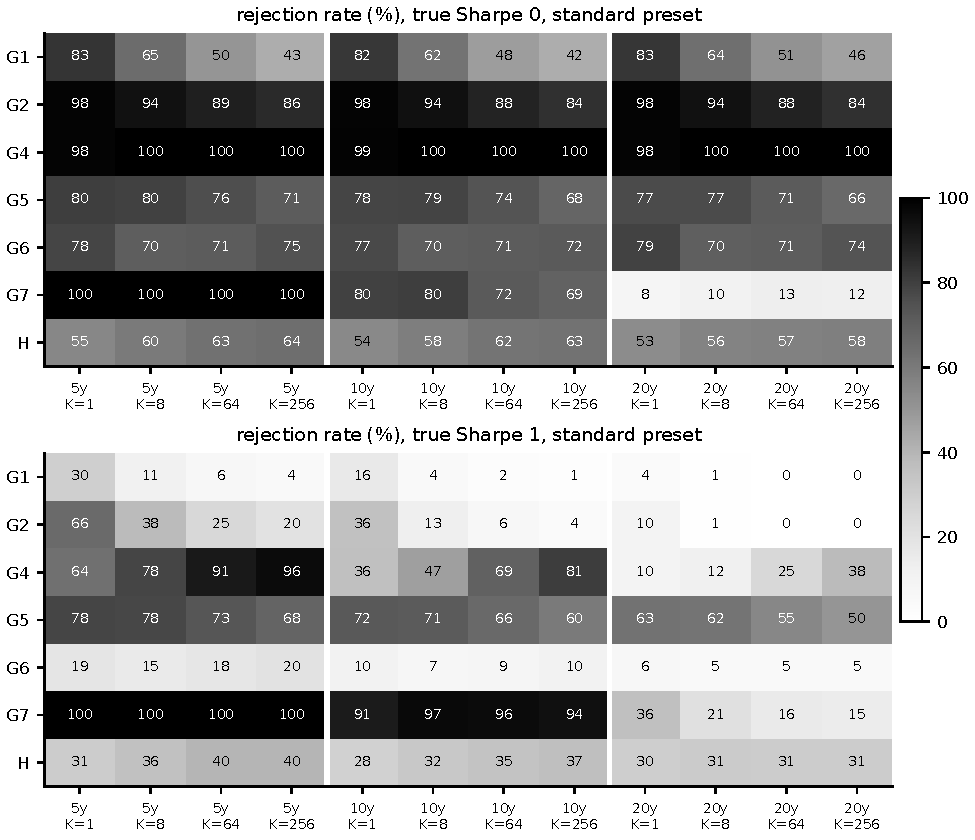
\includegraphics[width=\linewidth]{figures/fig10_gate_heat.pdf}
\caption{Per-gate rejection rates (\%) of the selected configuration, iid $t_5$ data, standard preset, by training length (years) and search size K. Top: noise (a rejection is correct); bottom: a planted Sharpe of 1 (a rejection is a miss). M = 2000 paths per cell; the Monte-Carlo se is at most 1.1 percentage points.}
\label{fig:fig10_gate_heat}
\end{figure}

Figure~\ref{fig:fig10_gate_heat} shows which gate rejects. Under noise, G4 rejects almost every
selection on its own; G2 and the other gates add little. With a real edge the binding gates change: G7
rejects nearly all five- and ten-year selections (a rule that changes position about eight times a year
rarely reaches 100 closed trades in ten years), G5 rejects at least half of the selections at every length,
and G4 rejects more as $K$ grows. G1 and G6 bind mainly for five years; with a Sharpe ratio of 1 and 10 or
20 years they pass in 84\,\% of the paths or more. G2 binds longer: with $K = 1$ it still rejects 36\,\% of
the ten-year selections (10\,\% with 20 years); with $K \ge 64$ it passes 94\,\% or more from ten years on.

\subsection{Power}
\begin{figure}[H]
\centering
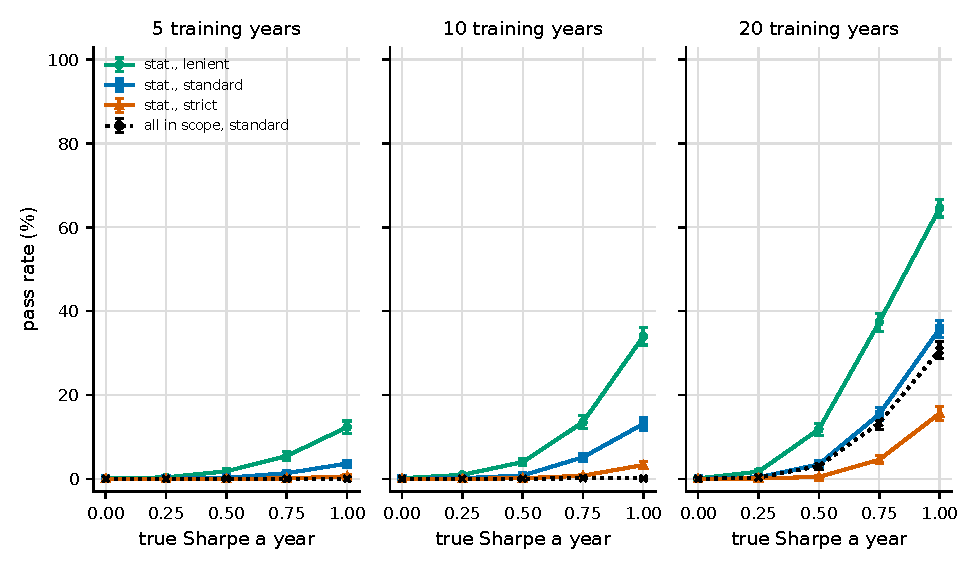
\includegraphics[width=\linewidth]{figures/fig9_power.pdf}
\caption{Power curves: pass rate of the best of K = 64 configurations against the true (gross) Sharpe ratio of the planted configuration, iid $t_5$ data, per training length. Coloured: the statistical gates per preset; dotted black: all in-scope gates including G7 (standard). The value at Sharpe 0 is the false-positive rate. M = 2000 paths per point, error bars $\pm 1.96$ se.}
\label{fig:fig9_power}
\end{figure}

\begin{table}[H]
\centering
\scriptsize
\caption{Power (\%): pass rate of the best of $K$ = 64 configurations when the true configuration has the given gross Sharpe ratio a year. Statistical gates per preset and all in-scope gates (standard). M = 2000 paths per cell, $\pm$ Monte-Carlo se; a rate of 0 or 100 shows the 95\,\% bound of the rule of three in brackets (3 / n).}
\label{tab:O3_power}
\setlength{\tabcolsep}{3pt}
\begin{tabular}{llrrrrr}
\toprule
Gates & Data & Years & SR 0.25 & SR 0.5 & SR 0.75 & SR 1 \\
\midrule
Stat., lenient & iid $t_5$ & 5 & 0.4 $\pm$ 0.1 & 1.8 $\pm$ 0.3 & 5.5 $\pm$ 0.5 & 12.3 $\pm$ 0.7 \\
Stat., lenient & iid $t_5$ & 10 & 0.9 $\pm$ 0.2 & 4.0 $\pm$ 0.4 & 13.5 $\pm$ 0.8 & 34.0 $\pm$ 1.1 \\
Stat., lenient & iid $t_5$ & 20 & 1.7 $\pm$ 0.3 & 11.8 $\pm$ 0.7 & 37.4 $\pm$ 1.1 & 64.5 $\pm$ 1.1 \\
Stat., lenient & GARCH-$t_5$ & 5 & 0.5 $\pm$ 0.2 & 1.9 $\pm$ 0.3 & 6.0 $\pm$ 0.5 & 14.2 $\pm$ 0.8 \\
Stat., lenient & GARCH-$t_5$ & 10 & 0.8 $\pm$ 0.2 & 4.3 $\pm$ 0.5 & 14.7 $\pm$ 0.8 & 36.9 $\pm$ 1.1 \\
Stat., lenient & GARCH-$t_5$ & 20 & 1.7 $\pm$ 0.3 & 12.3 $\pm$ 0.7 & 39.6 $\pm$ 1.1 & 66.5 $\pm$ 1.1 \\
\midrule
Stat., standard & iid $t_5$ & 5 & 0 ($\le$ 0.15) & 0.2 $\pm$ 0.1 & 1.4 $\pm$ 0.3 & 3.6 $\pm$ 0.4 \\
Stat., standard & iid $t_5$ & 10 & 0.1 $\pm$ 0.1 & 0.8 $\pm$ 0.2 & 5.1 $\pm$ 0.5 & 13.1 $\pm$ 0.8 \\
Stat., standard & iid $t_5$ & 20 & 0.4 $\pm$ 0.1 & 3.5 $\pm$ 0.4 & 15.4 $\pm$ 0.8 & 35.8 $\pm$ 1.1 \\
Stat., standard & GARCH-$t_5$ & 5 & 0.1 $\pm$ 0.0 & 0.2 $\pm$ 0.1 & 1.2 $\pm$ 0.2 & 4.4 $\pm$ 0.5 \\
Stat., standard & GARCH-$t_5$ & 10 & 0.1 $\pm$ 0.1 & 1.3 $\pm$ 0.3 & 4.8 $\pm$ 0.5 & 15.0 $\pm$ 0.8 \\
Stat., standard & GARCH-$t_5$ & 20 & 0.3 $\pm$ 0.1 & 3.7 $\pm$ 0.4 & 17.9 $\pm$ 0.9 & 37.0 $\pm$ 1.1 \\
\midrule
Stat., strict & iid $t_5$ & 5 & 0 ($\le$ 0.15) & 0 ($\le$ 0.15) & 0.1 $\pm$ 0.1 & 0.6 $\pm$ 0.2 \\
Stat., strict & iid $t_5$ & 10 & 0 ($\le$ 0.15) & 0.1 $\pm$ 0.1 & 0.8 $\pm$ 0.2 & 3.3 $\pm$ 0.4 \\
Stat., strict & iid $t_5$ & 20 & 0.1 $\pm$ 0.1 & 0.4 $\pm$ 0.1 & 4.5 $\pm$ 0.5 & 15.6 $\pm$ 0.8 \\
Stat., strict & GARCH-$t_5$ & 5 & 0 ($\le$ 0.15) & 0 ($\le$ 0.15) & 0.1 $\pm$ 0.1 & 0.7 $\pm$ 0.2 \\
Stat., strict & GARCH-$t_5$ & 10 & 0 ($\le$ 0.15) & 0.1 $\pm$ 0.0 & 0.9 $\pm$ 0.2 & 3.5 $\pm$ 0.4 \\
Stat., strict & GARCH-$t_5$ & 20 & 0 ($\le$ 0.15) & 0.6 $\pm$ 0.2 & 4.7 $\pm$ 0.5 & 16.1 $\pm$ 0.8 \\
\midrule
All, standard & iid $t_5$ & 5 & 0 ($\le$ 0.15) & 0 ($\le$ 0.15) & 0 ($\le$ 0.15) & 0 ($\le$ 0.15) \\
All, standard & iid $t_5$ & 10 & 0 ($\le$ 0.15) & 0 ($\le$ 0.15) & 0.1 $\pm$ 0.1 & 0.1 $\pm$ 0.1 \\
All, standard & iid $t_5$ & 20 & 0.3 $\pm$ 0.1 & 3.0 $\pm$ 0.4 & 13.3 $\pm$ 0.8 & 30.6 $\pm$ 1.0 \\
All, standard & GARCH-$t_5$ & 5 & 0 ($\le$ 0.15) & 0 ($\le$ 0.15) & 0 ($\le$ 0.15) & 0 ($\le$ 0.15) \\
All, standard & GARCH-$t_5$ & 10 & 0 ($\le$ 0.15) & 0.1 $\pm$ 0.0 & 0 ($\le$ 0.15) & 0.1 $\pm$ 0.0 \\
All, standard & GARCH-$t_5$ & 20 & 0.2 $\pm$ 0.1 & 2.9 $\pm$ 0.4 & 14.8 $\pm$ 0.8 & 26.4 $\pm$ 1.0 \\
\bottomrule
\end{tabular}
\end{table}

The price of this protection is power (Figure~\ref{fig:fig9_power}, Table~\ref{tab:O3_power}). With a
true Sharpe ratio of 1.0 and $K = 64$, the statistical gates with the standard preset pass about 4\,\% of
the selections with 5 training years, 13\,\% with 10 and 36\,\% with 20; the lenient preset 12, 34 and
65\,\%, the strict one 1, 3 and 16\,\%. With G7 included, the standard preset passes almost nothing below
20 years. Edges of a Sharpe ratio of 0.5 or less are confirmed in at most a few per cent of the paths, even
with 20 years.
\usertext{Is this power acceptable? Which edge size should the platform be able to confirm, and with how
many years of data?}

\subsection{The holdout}
\begin{figure}[H]
\centering
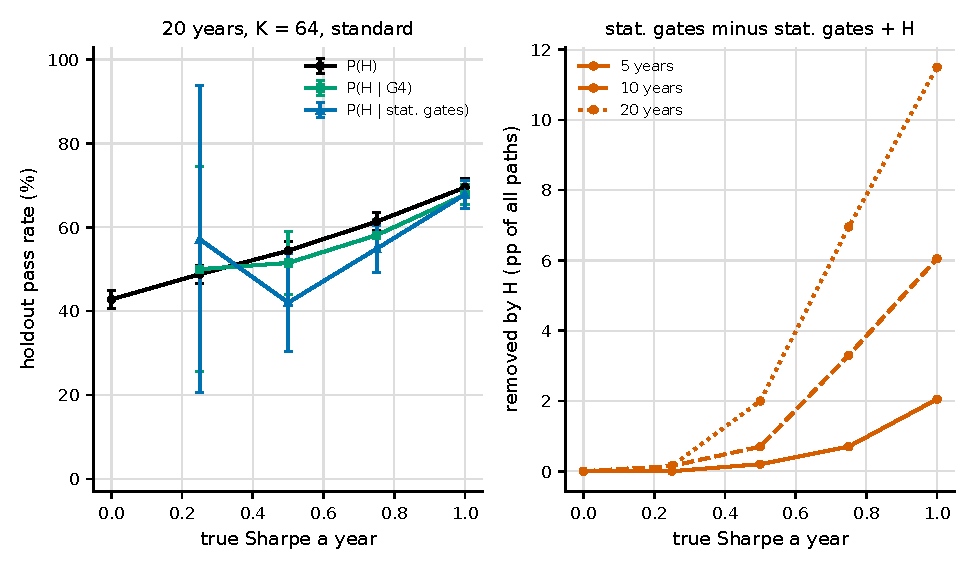
\includegraphics[width=\linewidth]{figures/fig11_holdout.pdf}
\caption{Value of the holdout gate H (24 months, evaluated once), iid $t_5$ data, best of K = 64, standard preset. Left: H pass rate unconditionally and among the paths that passed G4 or all statistical gates (points with no passing path are omitted). Right: the share of all paths that pass the statistical gates but fail H: under noise this is the holdout's gain, under a real edge its cost. M = 2000 paths per point, error bars $\pm 1.96$ se (conditional rates: on the passing paths only).}
\label{fig:fig11_holdout}
\end{figure}

\begin{table}[H]
\centering
\scriptsize
\caption{Value of the holdout gate H (20 training years, best of $K$ = 64, standard preset): the unconditional H pass rate, the conditional rates given G4 and given the statistical gates (number of passing paths in brackets), and the statistical gates without and with H. M = 2000 paths per cell, rates in \%, $\pm$ Monte-Carlo se; a rate of 0 or 100 shows the 95\,\% bound of the rule of three in brackets (3 / n).}
\label{tab:O4_holdout}
\setlength{\tabcolsep}{3pt}
\begin{tabular}{lrrrrrr}
\toprule
Data & True SR & P(H) & P(H $\mid$ G4) (n) & P(H $\mid$ stat.) (n) & Stat. & Stat. + H \\
\midrule
iid $t_5$ & 0 & 42.8 $\pm$ 1.1 & -- (0) & -- (0) & 0 ($\le$ 0.15) & 0 ($\le$ 0.15) \\
iid $t_5$ & 0.25 & 48.8 $\pm$ 1.1 & 50.0 $\pm$ 12.5 (16) & 57.1 $\pm$ 18.7 (7) & 0.4 $\pm$ 0.1 & 0.2 $\pm$ 0.1 \\
iid $t_5$ & 0.5 & 54.4 $\pm$ 1.1 & 51.5 $\pm$ 3.9 (167) & 42.0 $\pm$ 5.9 (69) & 3.5 $\pm$ 0.4 & 1.5 $\pm$ 0.3 \\
iid $t_5$ & 0.75 & 61.4 $\pm$ 1.1 & 58.1 $\pm$ 1.9 (702) & 54.9 $\pm$ 2.8 (308) & 15.4 $\pm$ 0.8 & 8.5 $\pm$ 0.6 \\
iid $t_5$ & 1 & 69.5 $\pm$ 1.0 & 67.8 $\pm$ 1.2 (1495) & 67.8 $\pm$ 1.7 (715) & 35.8 $\pm$ 1.1 & 24.2 $\pm$ 1.0 \\
\midrule
GARCH-$t_5$ & 0 & 42.1 $\pm$ 1.1 & -- (0) & -- (0) & 0 ($\le$ 0.15) & 0 ($\le$ 0.15) \\
GARCH-$t_5$ & 0.25 & 49.0 $\pm$ 1.1 & 38.9 $\pm$ 11.5 (18) & 33.3 $\pm$ 19.2 (6) & 0.3 $\pm$ 0.1 & 0.1 $\pm$ 0.1 \\
GARCH-$t_5$ & 0.5 & 56.5 $\pm$ 1.1 & 53.7 $\pm$ 3.6 (188) & 47.3 $\pm$ 5.8 (74) & 3.7 $\pm$ 0.4 & 1.8 $\pm$ 0.3 \\
GARCH-$t_5$ & 0.75 & 64.4 $\pm$ 1.1 & 59.2 $\pm$ 1.7 (809) & 58.5 $\pm$ 2.6 (359) & 17.9 $\pm$ 0.9 & 10.5 $\pm$ 0.7 \\
GARCH-$t_5$ & 1 & 71.0 $\pm$ 1.0 & 69.0 $\pm$ 1.2 (1573) & 65.7 $\pm$ 1.7 (740) & 37.0 $\pm$ 1.1 & 24.3 $\pm$ 1.0 \\
\bottomrule
\end{tabular}
\end{table}

H is a separate sample, but its 50\,\%-of-training clause makes it harder to pass for selections with high
training Sharpe ratios (Figure~\ref{fig:fig11_holdout}, Table~\ref{tab:O4_holdout}): among the paths that pass
the statistical gates, H passes less often than unconditionally (with 20 years, $K = 64$ and a true Sharpe
ratio of 0.75: 54.9 against 61.4\,\%, about 2 se apart), because the selections that pass have high training
Sharpe ratios, partly by luck (the winner's curse), and the clause asks for half of that. With 24 months the holdout Sharpe ratio has a standard error of about 0.7, so H passes
about 40\,\% of noise selections and about 70\,\% of selections with a true Sharpe ratio of 1. Because the
statistical gates already let almost no noise through, H removes practically no false positives in this
setting but about a third of the true positives (20 years, Sharpe 1.0: from 36\,\% to 24\,\%).

\subsection{Calibration of SPEC \S 9.6}
\begin{table}[H]
\centering
\scriptsize
\caption{Calibration claims of SPEC \S 9.6 on noise (standard preset): share of noise paths that fail at least one in-scope gate (claim: $\ge$ 95\,\%) and share of best-of-64 noise selections that fail G4 or G5 (claim: all). M = 2000 paths per cell, \%, $\pm$ Monte-Carlo se; a rate of 0 or 100 shows the 95\,\% bound of the rule of three in brackets (3 / n).}
\label{tab:O5_calibration}
\begin{tabular}{lrrrrr}
\toprule
Data & Years & Fail $\ge$1, $K$=64 & Fail G4/G5, $K$=64 & Fail $\ge$1, $K$=256 & Fail G4/G5, $K$=256 \\
\midrule
iid $t_5$ & 5 & 100 ($\ge$ 99.85) & 100.0 $\pm$ 0.0 & 100 ($\ge$ 99.85) & 100 ($\ge$ 99.85) \\
iid $t_5$ & 10 & 100 ($\ge$ 99.85) & 100 ($\ge$ 99.85) & 100 ($\ge$ 99.85) & 100 ($\ge$ 99.85) \\
iid $t_5$ & 20 & 100 ($\ge$ 99.85) & 100 ($\ge$ 99.85) & 100 ($\ge$ 99.85) & 100.0 $\pm$ 0.0 \\
GARCH-$t_5$ & 5 & 100 ($\ge$ 99.85) & 100 ($\ge$ 99.85) & 100 ($\ge$ 99.85) & 100 ($\ge$ 99.85) \\
GARCH-$t_5$ & 10 & 100 ($\ge$ 99.85) & 100 ($\ge$ 99.85) & 100 ($\ge$ 99.85) & 100 ($\ge$ 99.85) \\
GARCH-$t_5$ & 20 & 100 ($\ge$ 99.85) & 100 ($\ge$ 99.85) & 100 ($\ge$ 99.85) & 100 ($\ge$ 99.85) \\
\bottomrule
\end{tabular}
\end{table}

The first calibration claim of SPEC \S 9.6 holds for this rule family (Table~\ref{tab:O5_calibration}): at
least 99.6\,\% of the noise selections fail at least one in-scope gate in every cell, and all best-of-64 noise
selections do (the claim is at least 95\,\%). The second claim, that every best-of-64 noise selection fails G4
or G5, fails narrowly: one of the 12\,000 best-of-64 noise selections (iid data, 5 years) passed both G4 and
G5; it failed another in-scope gate. A rate of 0 or 100\,\% is shown with the 95\,\% bound of the rule of
three ($3/M$ = 0.15 percentage points for $M = 2000$).

% =====================================================================================
\section{Limitations}
\begin{itemize}
\item One rule family (moving-average crossovers on one asset) and one cost level; families whose
  configurations are less correlated, or cross-sectional strategies, can behave differently, in particular
  for G4 ($N = K + 1$ treats correlated trials as independent) and G5.
\item The true configuration lies inside the search space and the edge is a constant drift times its
  position; real edges decay, switch on and off and are shared imperfectly by neighbouring configurations.
\item Out of scope: G1's rank-IC form, G3, the cost and stress parts of G6, G8. The platform's decision for
  a real strategy also depends on them.
\item The family's trials are the searched configurations only; earlier, unrecorded searches of a user
  would raise the true $N$ and are not modelled.
\item Synthetic data with Student-$t$ innovations, iid or GARCH(1,1); no regime changes, no jumps, no
  transaction-cost uncertainty. The $\pm$ se are Monte-Carlo noise only.
\end{itemize}
\usertext{Further limitations the author sees, and how they affect the conclusions.}

% =====================================================================================
\section{Findings}
\begin{table}[H]
\centering
\scriptsize
\caption{Findings register of the gate overfitting study. Severities are PROPOSED and must be confirmed by the validator.}
\label{tab:O6_findings}
\setlength{\tabcolsep}{3pt}
\begin{tabular}{>{\raggedright\arraybackslash}p{0.75cm}>{\raggedright\arraybackslash}p{6.8cm}>{\raggedright\arraybackslash}p{1.85cm}>{\raggedright\arraybackslash}p{2.2cm}>{\raggedright\arraybackslash}p{3.5cm}}
\toprule
ID & Finding & Severity & Evidence & Proposed remediation \\
\midrule
O-F1 & The gates control false positives of a searched noise rule: the statistical gates pass at most 1.9 $\pm$ 0.3\,\% of noise selections in any cell (lenient, 10 years, $K$ = 1); standard preset at most 0.5 $\pm$ 0.2\,\%. Single gates leak much more: G1 passes 57.8 $\pm$ 1.1\,\% and H 37.2 $\pm$ 1.1\,\% of best-of-256 noise (10 years). & PROPOSED: Low & Tab.~\ref{tab:O2_fpr}; Fig.~\ref{fig:fig8_fpr_vs_k}, \ref{fig:fig10_gate_heat} & Keep the conjunction of gates; do not relax G4 / G5 to a single-gate screen. \\
O-F2 & Low power for a genuine but modest edge: with a true Sharpe of 1.0 and $K$ = 64 the statistical gates (standard) pass 13.1 $\pm$ 0.8\,\% with 10 training years and 35.8 $\pm$ 1.1\,\% with 20; all in-scope gates 0.1 $\pm$ 0.1\,\% and 30.6 $\pm$ 1.0\,\%. & PROPOSED: High & Tab.~\ref{tab:O3_power}; Fig.~\ref{fig:fig9_power} & State the power in the UI next to the presets (a pass is rare even for a real Sharpe of 1); consider the lenient preset for long samples only together with H. \\
O-F3 & G5 (PBO) rejects real edges shared by a correlated family: with a true Sharpe of 1.0 and $K$ = 64, G5 passes only 26.7, 33.7, 44.5\,\% (5 / 10 / 20 years, standard), against 23.8, 26.2, 28.8\,\% under noise: G5 barely separates the two. The planted edge lifts all neighbouring configurations, so the in-sample winner is close to a coin flip out of sample within the grid; PBO measures the stability of the ranking, not the existence of an edge. & PROPOSED: Medium & Tab.~\ref{tab:O3_power}; Fig.~\ref{fig:fig10_gate_heat} & Document that G5 tests the selection within the grid; consider reporting PBO beside a test of the grid's median Sharpe instead of as a hard gate for smooth families. \\
O-F4 & G4 power falls with the search size even for a real edge: with a true Sharpe of 1.0 and 20 years, G4 passes 89.8, 87.8, 74.8, 62.0\,\% for $K$ = 1, 8, 64, 256 (standard). $N = K + 1$ counts every tried configuration as an independent trial. The selection's training Sharpe is consistent with strongly correlated trials: under noise the best of 64 has a mean training Sharpe of 0.34 (10 years), against 0.75 expected for 64 independent trials. (No effective trial count was estimated in this study.) & PROPOSED: Medium & Fig.~\ref{fig:fig10_gate_heat}; results file & Consider an effective number of trials for correlated families (e.g. from the trials' correlation) and record how $N$ was counted. \\
O-F5 & G7 (closed trades) is decided by the rule's trading frequency and the sample length, not by overfitting: the noise selections pass G7 in 0.0, 28.2, 86.7\,\% of paths for 5, 10, 20 years (standard, mean 40, 81, 168 trades). & PROPOSED: Medium & Results file (pass\_G7, trades\_mean) & Scale the minimum trade count with the sample length or the holding period. \\
O-F6 & The holdout gate mostly costs power here: H alone passes 38.1 $\pm$ 1.1\,\% of best-of-64 noise (10 years) and 69.5 $\pm$ 1.0\,\% with a true Sharpe of 1.0 (20 years); 24 months give a Sharpe standard error of about 0.7. H is a separate sample, but its 50\,\%-of-training clause makes it harder to pass for selections with high training Sharpe ratios: among the selections that pass the statistical gates (20 years, $K$ = 64), H passes 54.9 $\pm$ 2.8\,\% against 61.4 $\pm$ 1.1\,\% unconditionally at a true Sharpe of 0.75, and 67.8 $\pm$ 1.7\,\% against 69.5 $\pm$ 1.0\,\% at 1.0. Behind the statistical gates, whose false-positive rate is already near 0, H cuts the power at a true Sharpe of 1.0 (20 years, $K$ = 64) from 35.8 $\pm$ 1.1\,\% to 24.2 $\pm$ 1.0\,\%. & PROPOSED: Medium & Tab.~\ref{tab:O4_holdout}; Fig.~\ref{fig:fig11_holdout} & Treat H as a sanity check, not as evidence; a longer holdout or a pooled out-of-sample record adds more. \\
O-F7 & SPEC \S 9.6 calibration: of the best-of-64 noise selections (standard), all 2000 (95\,\% lower bound of the rate 99.85\,\%) fail at least one in-scope gate in every cell (claim: $\ge$ 95\,\%). The claim that every best-of-64 noise selection fails G4 or G5 fails narrowly: 1 of 12000 selection(s) passed both G4 and G5 (lowest cell 99.95\,\% fail G4 or G5); those selection(s) failed another in-scope gate. The selected configuration has a grid neighbour in at least 84.4\,\% of the paths of every cell. & PROPOSED: Low & Tab.~\ref{tab:O5_calibration} & None for the claims; extend the study to G3, the G6 cost / stress parts and G8. \\
\bottomrule
\end{tabular}
\end{table}

\usertext{Validator's confirmation or change of the proposed severities, and the owner of each remediation.}

% =====================================================================================
\section*{References}
\begin{itemize}
\item Bailey, D. H., Borwein, J. M., L\'opez de Prado, M. and Zhu, Q. J. (2017). The probability of backtest
  overfitting. \emph{Journal of Computational Finance} 20(4), 39--69.
\item Bailey, D. H. and L\'opez de Prado, M. (2012). The Sharpe ratio efficient frontier. \emph{Journal of
  Risk} 15(2), 3--44.
\item Bailey, D. H. and L\'opez de Prado, M. (2014). The deflated Sharpe ratio: correcting for selection
  bias, backtest overfitting and non-normality. \emph{Journal of Portfolio Management} 40(5), 94--107.
\item Lo, A. W. (2002). The statistics of Sharpe ratios. \emph{Financial Analysts Journal} 58(4), 36--52.
\item Newey, W. K. and West, K. D. (1987). A simple, positive semi-definite, heteroskedasticity and
  autocorrelation consistent covariance matrix. \emph{Econometrica} 55(3), 703--708.
\item Newey, W. K. and West, K. D. (1994). Automatic lag selection in covariance matrix estimation.
  \emph{Review of Economic Studies} 61(4), 631--653.
\end{itemize}

\appendix
\section{Reproduction}
From \texttt{UFOS.ai/RiskLab/}:
\begin{verbatim}
python studies/gate_overfitting.py --mode full --save-results
python report/build_report.py --doc overfitting
# -> out/report/overfitting_study.pdf
\end{verbatim}
The study writes \texttt{studies/results/gate\_overfitting\_full\_results.json} (with the code fingerprint and
the package versions) and the summary next to it; the build regenerates figures 8--11 and tables O1--O6
from it.

\end{document}
